We have conducted two different experiments, one to predict the force measured
by the force sensor and another one to classify the grasp type.
The EMG data were the preprocessed as described in Sec ???.
To assess the performance of the proposed adaptation method we have compared it
to two baseline methods. The first one consists in using only the stored models
wihtout updating them; the second one consists in using only the new data for
training. The parameters of the training ($C$ and $\gamma$) were chosen by
cross-validation.

Given that we have data from $10$ subjects we have used a sort of
cross-validation to test the methods. In particular we consider one of the
subject for the new data and use the other $9$ subjects to train the stored
models. We repeat this procedure $10$ times, one for each subject, to have a
reliable estimation of the performance.

\begin{figure}[t]
  \centering
  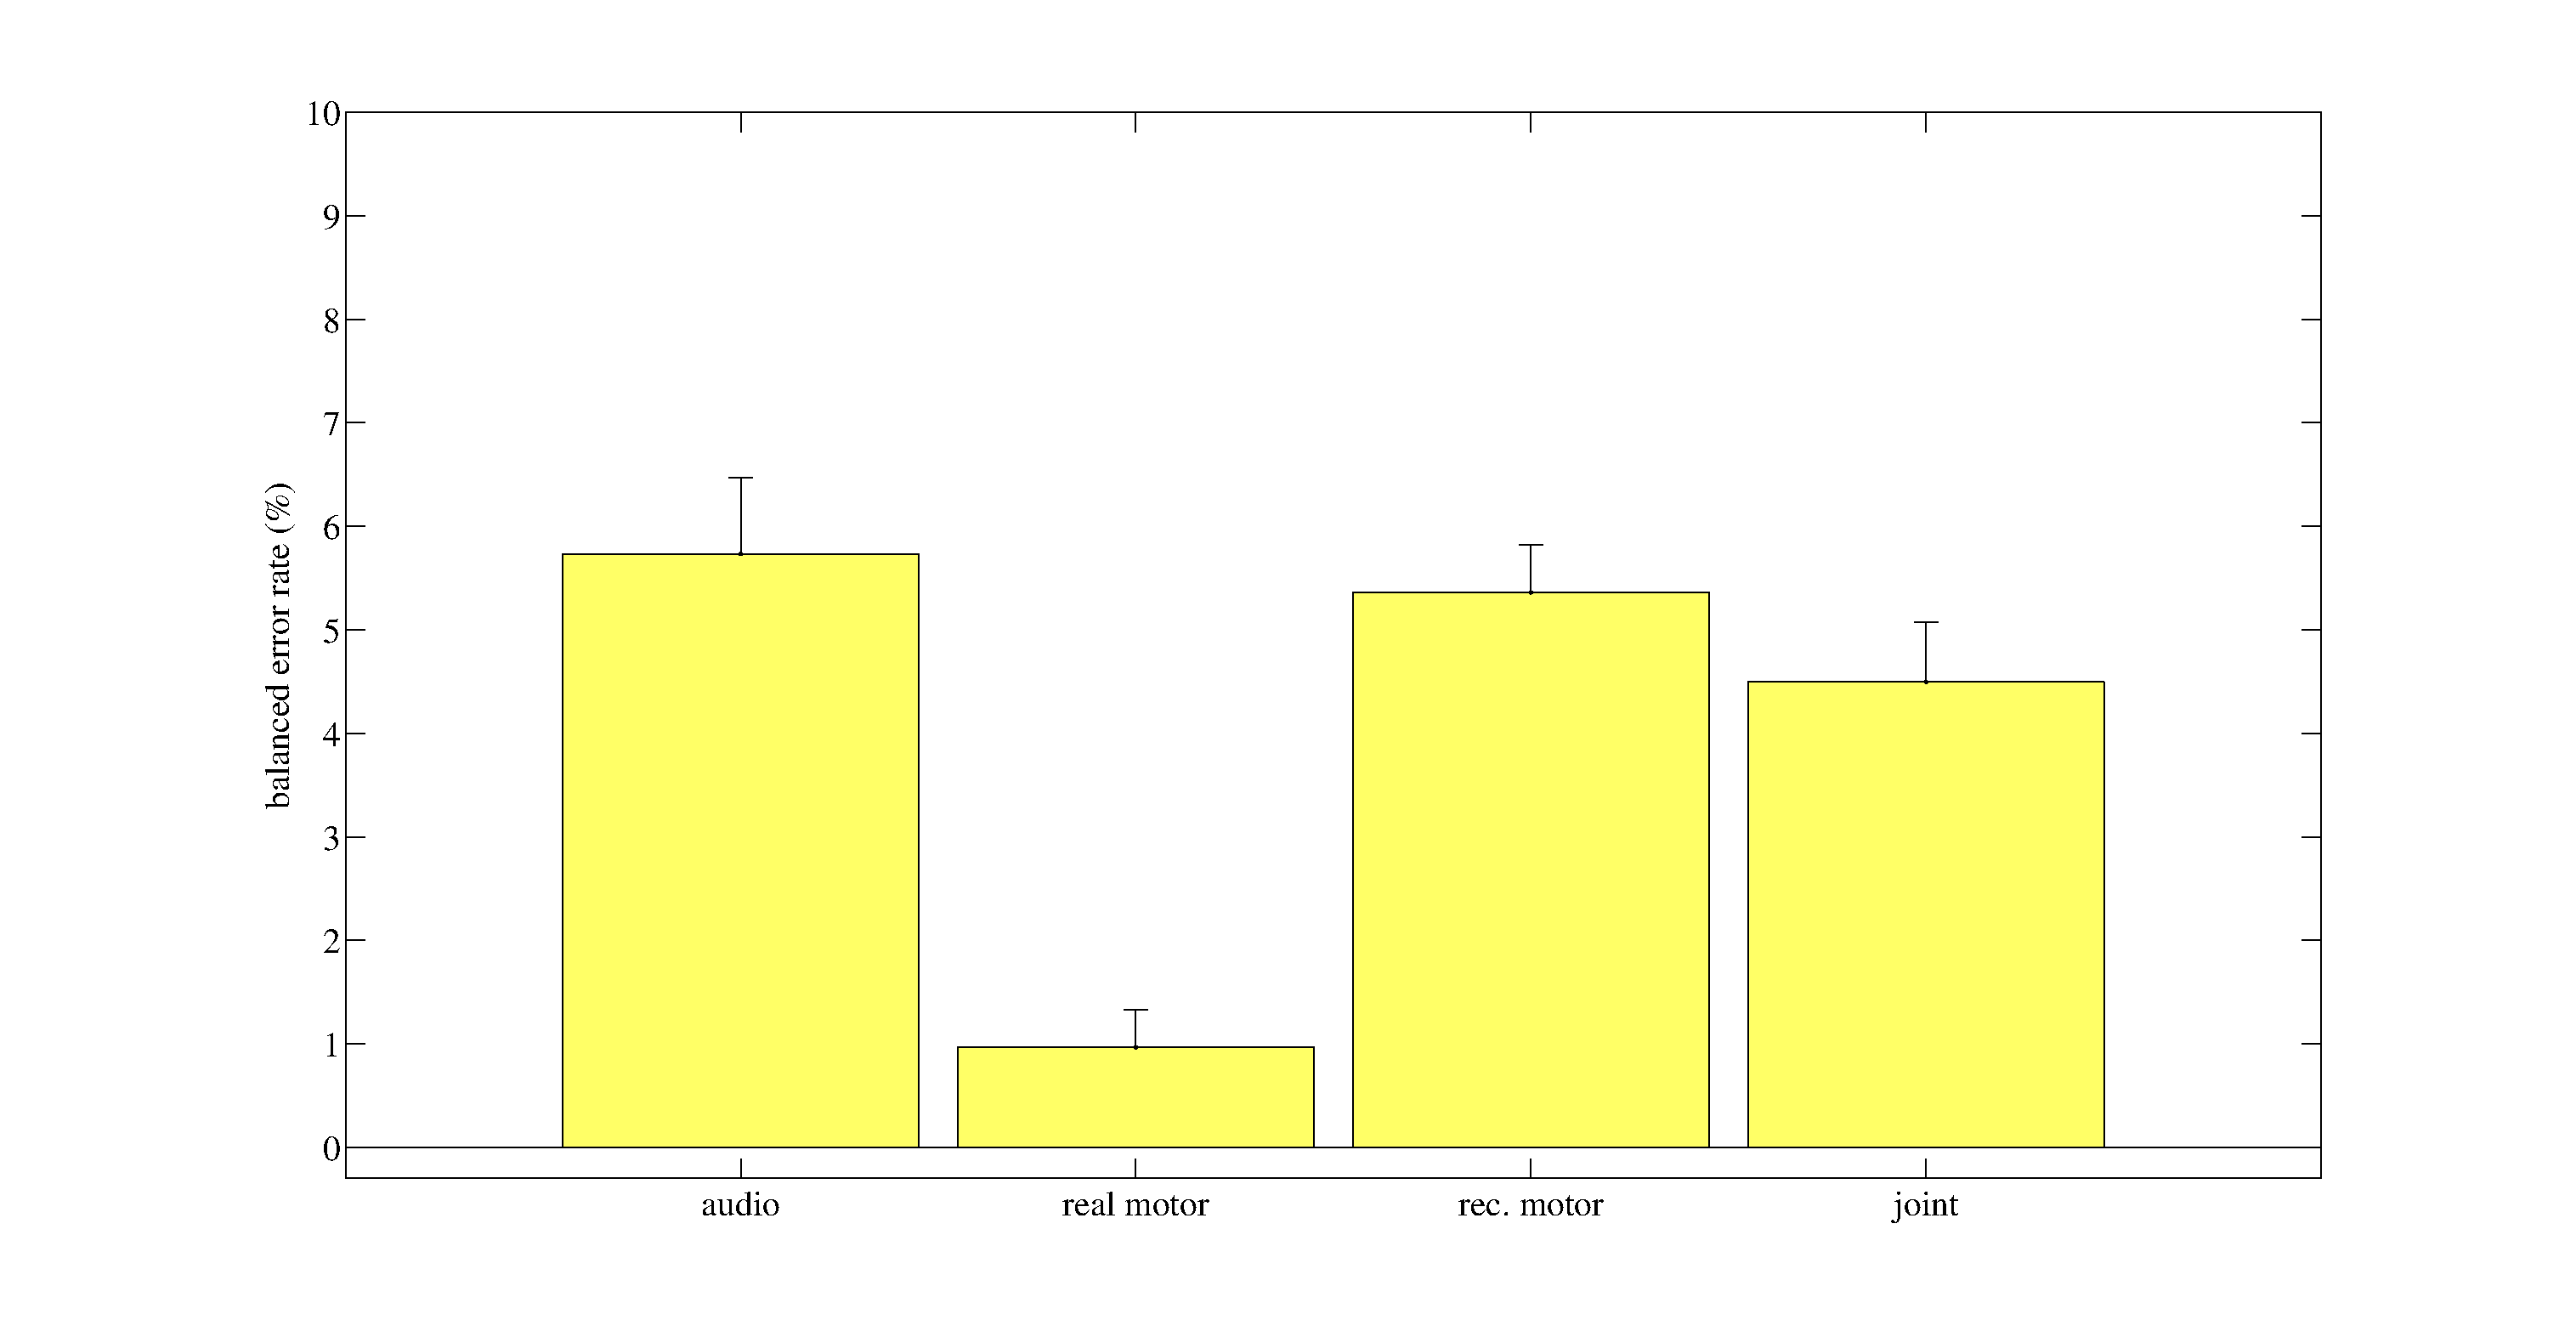
\includegraphics[width=0.95\linewidth]{figs/exp1}
  \caption{The classification experiment.}
  \label{fig:exp1}
\end{figure}

\begin{figure}[t]
  \centering
  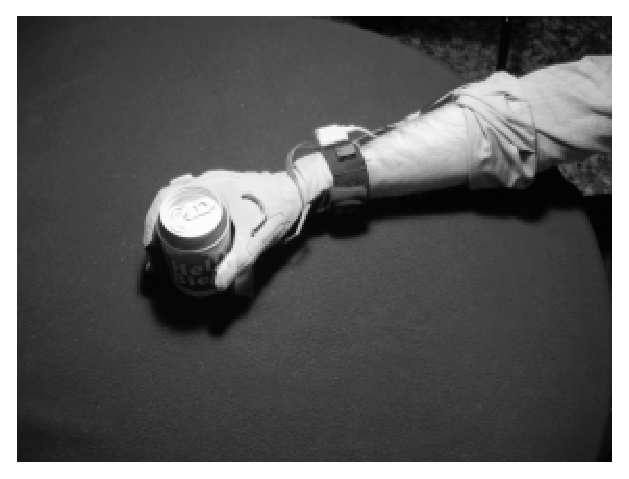
\includegraphics[width=0.95\linewidth]{figs/exp2}
  \caption{The regression experiment.}
  \label{fig:exp2}
\end{figure}